
\subsection{Monochromatic filters}
Let $W \in \mathbb{R}^{C \times X \times Y \times F}$ denote the first convolutional layer weights of a trained network. The number of input channels, $C$, is 3 and each channel corresponds to a different color component (either RGB or YUV). We found that the color components of weights from a trained convolutional neural network have low dimensional structure. In particular, the weights can be well approximated by projecting the color dimension down into a 1D subspace. Figure ?? shows the original first layer convolutional weights of a trained network and the weights after the color dimension has been projected into 1D lines. 

The approximation for this layer exploits this low dimensional structure and is computed as follows. First, for every output feature, $f$, we consider consider the matrix $W_f \in \mathbb{R}^{C \times XY }$, where the spatial dimensions of the filter corresponding to the output feature have been combined, and find the singular value decomposition, 
\begin{equation*}
	W_f = U_f S_f V_f^{\top}
\end{equation*}
where $U_f \in \mathbb{R}^{C \times C}, S_f \in \mathbb{R}^{C \times XY}, V_f \in \mathbb{R}^{XY \times XY}$. We then take the rank 1 approximation to $W_f$ 
\begin{equation*}
	\tilde{W}_f = \tilde{U}_f \tilde{S}_f \tilde{V}_f^{\top}
\end{equation*}
where $\tilde{U}_f \in \mathbb{R}^{C \times 1}, \tilde{S}_f \in \mathbb{R}, \tilde{V}_f \in \mathbb{R}^{1 \times XY}$.

This approximation corresponds to shifting from $C$ color channels to 1 color channel for each output feature. We can further exploit the regularity in the weights by sharing the color component basis between different output features. We do this by clustering the $F$ left singular vectors,  $\tilde{U}_f$, of each output feature $f$ into $C'$ equal sized clusters, where $C'$ is much smaller than $F$. Then, for each of the $\frac{F}{C'}$ output features, $f$, that is assigned to cluster $c$, we can approximate $W_f$ with
\begin{equation*}
	\tilde{W}_f = U_c \tilde{S}_f \tilde{V}_f^{\top}
\end{equation*}
where $U_c \in \mathbb{R}^{C \times 1}$ is the cluster center for cluster $c$ and $\tilde{S}_f$ and $\tilde{V}_f$ as as before. 

By decomposing the approximated weights into two tensors, this low-rank approximation allows for a more efficient computation of the convolutional layer output. Let $W_C \in \mathbb{R}^{C' \times C}$ denote the color transform matrix where the rows of $W_c$ are the cluster centers $U_c^{\top}$. Let $W_{mono} \in \mathbb{R}^{X \times Y \times F}$ denote the monochromatic weight tensor containing $ \tilde{S}_f \tilde{V}_f^{\top}$ for each of the $F$ output features. Given this decomposition, we can compute the output of the convolutional layer by first transforming the input signal, $I \in \mathbb{R}^{C \times N \times M}$ into a different basis using the color transform matrix: 
\begin{equation*}
	\tilde{I} = W_c \otimes I
\end{equation*}
where $\tilde{I} \in \mathbb{R}^{C' \times N \times M}$. After the color transformation, each of the $f$ filters in $W_{mono}$ is monochromatic in the sense that it only acts upon one of the $C'$ color channels. The fact that we can do this approximation without hurting performance indicates that the structure inherent in the learned first convolutional layer weights of a network make it such that, in a new basis, the connections between input and output maps become sparse. To be specific, target value, $\tilde{T}$, of the approximated convolutional layer for a particular output feature $f$, and spatial location $(x, y)$ is
\begin{align*}
	\tilde{T}(f, x, y) &= \sum_{x' = 1}^{X} \sum_{y' = 1}^{Y} \Big(\sum_{c = 1}^{C} I(c, x + x', y + y') W_c(c', c) \Big) \\
			&\hspace{3mm} \times (c, x + x', y + y') W(x', y', f) \\
			&= \sum_{x' = 1}^{X} \sum_{y' = 1}^{Y} \tilde{I}(c', x + x', y + y') W(x', y', f)
\end{align*} 
where $c' \in [1, ..., C']$ is the cluster feature $f$ is assigned to. If the color transformation is computed once at the outset, then the number of operations performed is significantly reduced.  

\subsubsection{Complexity analysis}
By using the monochromatic filter approximation to the first layer convolutional weights, the target output can be computed with significantly fewer operations. The number of operations that will be required is a function the number of color components, $C'$, that are used in the approximation. Table \ref{monochromatic_ops} gives the number of operations required in the original and approximated cases as a function of $C'$. 

\begin{table}[h]
\tiny
\parbox{\linewidth}{
\centering
\begin{tabular}{cc}
\hline
Original & Approximated \\
\hline
$C X Y F N M \Delta^{-2}$  & $	 C' C^2 N M + X Y F N M \Delta^{-2}$\\
\hline
\end{tabular}
\caption{Number of operations required to compute target output of first convolutional layer with original weights vs. monochromatic approximation, where $\Delta$ is the stride of the filter.}
\label{monochromatic_ops}
}
\end{table}

Figure \ref{monochromatic_ops_pic} shows the relative reduction in operations for varying values of $C'$.

\begin{figure}[t]
\centering
\mbox{
  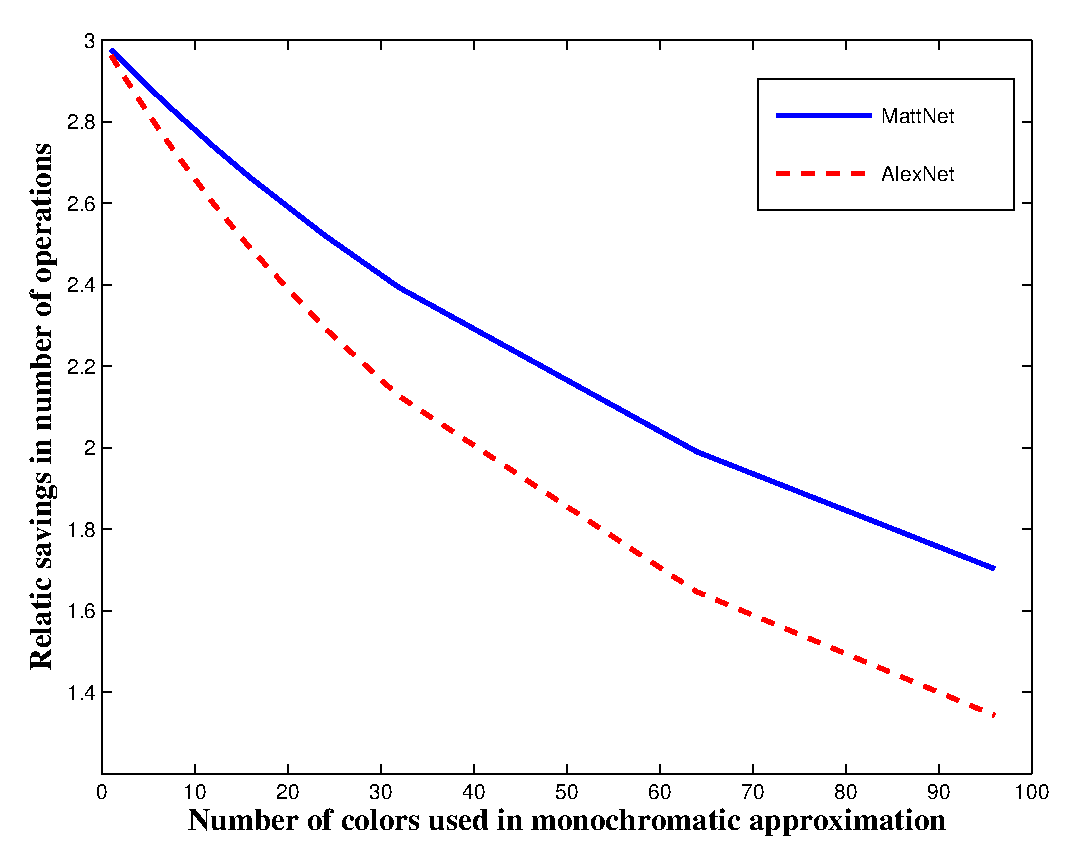
\includegraphics[width=0.75\linewidth]{img/monochromatic_numcolors_vs_numops.eps} 
}
\label{monochromatic_ops_pic}
\caption{Relative savings in number of operations required to compute output of first convolutional layer for various monochromatic approximations applied to MattNet (blue) and AlexNet (red).}
\end{figure}

\subsubsection{Empirical performance}
There is an obvious tradeoff between increased efficiency and decreased accuracy of the network as we approximate the filters with varying values of $C'$. In our experiments we only used approximations that did not increase the error of the network. However, it is insightful to see how test error varies with the number of color components used. Figure \ref{monochromatic_numcolors_vs_testerr} illustrates the tradeoff.

\begin{figure}[t]
\centering
\mbox{
  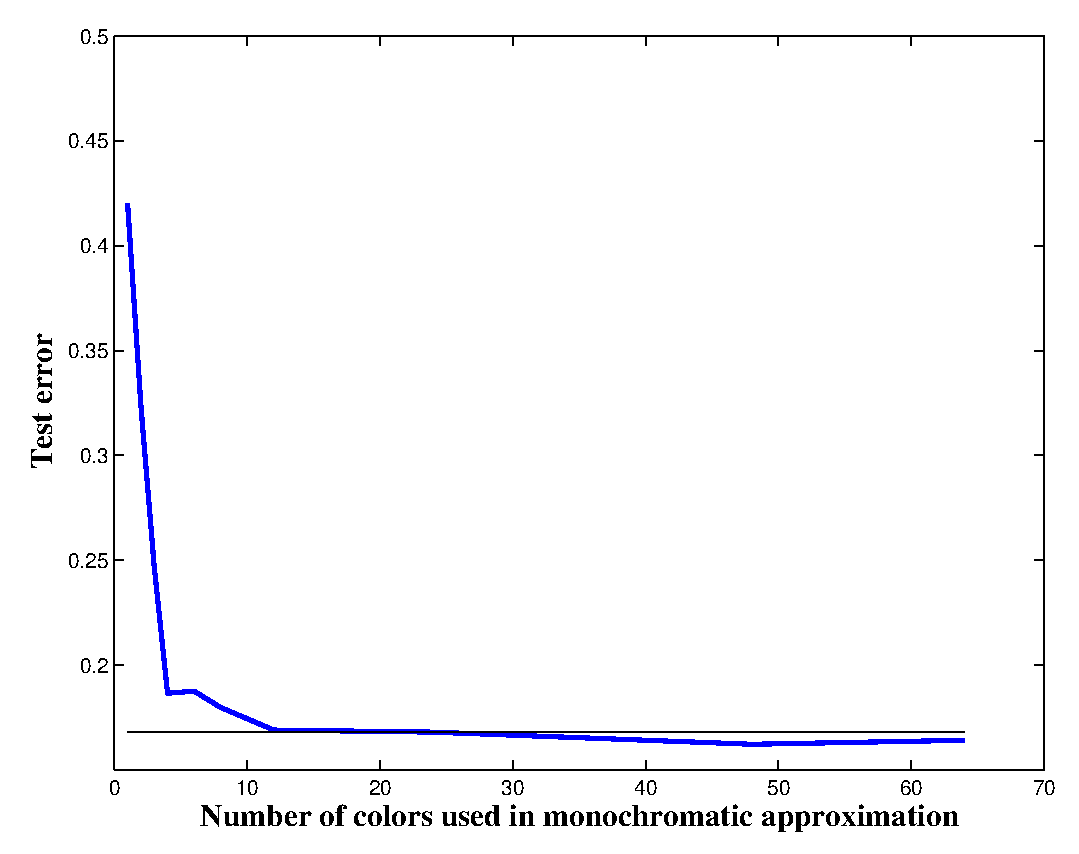
\includegraphics[width=0.75\linewidth]{img/layer1testerror_vs_numcolors.eps} 
}
\label{monochromatic_numcolors_vs_testerr}
\caption{Performance of MattNet as a function of the number of colors used the monochromatic approximation for for first layer weights.}
\end{figure}

